%!TEX root = ../../../report.tex
\section{The evolution of bipedalism}
\label{sec:bipedalism}

The current human bipedal locomotion arises from the combination of a wide variety of subsystems working in conjunction to achieve the intended gait generation according to the requirements of the situation.
The biomechanics of the limbs, consisting in bones, muscles and tendons under the control of the nervous system yields the adequate production of the different motion patterns in order to displace the body as energetically efficiently as possible.
This complex behavior is the result of 4 million years of an evolution \cite{bipedalism2} that started in primates and that has entailed both morphological and neurological changes in the human body since the first bipedal hominids to the current structure in Homo sapiens.
There exist several different theories about the reasons that originated and led to the adaption of this posture and bipedal motion.
Although different, most of them assume that most of them assume that the development of this structural and behavioral changes arose from a change in the environment in pre-hominids, for with bipedal behavior suddenly offered some kind of survival value \cite{bipedalism1}.
However, the genus Homo is not the only species that has evolved towards two-legged locomotion
Currently there are a few more species that have reached this method of displacement as a result of a natural selection process in which bipedalism offered the broadest set of advantages of the specie being the main ones listed below. 

\\
\hfill

\begin{itemize}
	\item Erect posture for a wider field of view and reach range.
	\item Free forelimbs, that could evolve towards specialized, non-locomotory applications such as object manipulation, combat, flight, etc.
	\item Faster displacement in certain species, although not generally.
\end{itemize}

Extensive research in the actuation and control structures involved in human bipedalism has been conducted from within the scientific fields of anthropology, biology, medicine, sport science and lately, several areas withing the engineering.
Its goal, as per definition of science, has been to reach a full understanding of what led to this behavior and the knowledge of how it functions, together with the discovery of ways in which it can be mimicked and improved, aiming at a more inexpensive and optimized locomotion.
This last fact has led to the belief that the next stage in the evolution of human locomotion will not come from nature as until nowadays, but from the hand of science and engineering, which has been lately depicted in literature and pop-culture as in \ref{fig:biped_evolution}.

\begin{figure}[h]
	\centering
	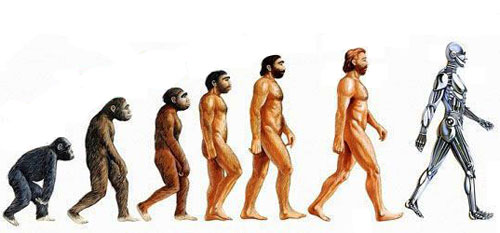
\includegraphics[width=0.8\textwidth]{figures/artificialhumans.jpg}
	\caption{Evolution of bipedalism (artistic depiction from \cite{human_evol_fig})}
	\label{fig:biped_evolution}
\end{figure}

\subsection{Biped motion and engineering} % (fold)
\label{sub:bipedalism_and_engineering}
The discipline of engineering has been historically among the latest of the cited ones to start its contribution to the research and improvement of biped motion in a well defined manner, although its earliest contributions seem to date from ancient Egypt and India \cite{prosthetics_history}.
From the study of human bipedal motion described above, the insights emerged regarding its biomechanical and control functioning together with the need to restore, improve or imitate its capabilities led to the creation of new branches within the discipline of engineering.
The three most relevant ones for the present thesis are listed and introduced below.

\begin{enumerate}
	\item Orthotics
	\item Prosthetics
	\item Artificial legged locomotion 
\end{enumerate}

\paragraph{Orthotics} % (fold)
\label{par:orthotics}
Orthotics is a specialty within the medical field concerned with the design, manufacture and application of orthoses. An orthosis is an externally applied device used to modify the structural and functional characteristics of the neuromuscular and skeletal system, as per definition in \cite{ISO_orthosis}.

Therapeutic models to exoskeletons... 
\todo{Add some more stuff}
% paragraph orthotics (end)

\paragraph{Prosthetics} % (fold)
\label{par:prosthetics}
Prosthetics is the field of medicine that comprises the design and creation of prosthesis, defined as artificial limbs aimed at restoring motor and sensory capabilities in amputee patients.
Since the first lower-limb prosthesis implant recorded in history, documented in the Rigveda \cite{prosthetics_history}, to the current state of the art there has been more than 3000 years of development.
This time has taken prosthetics from single-piece, non-articulated devices with no actuation or sensory feedback to the current near-natural, anthropomorphic structures and control systems adapted to the patient needs and able to closely provide the properties of a biological limb.
As in the orthoses design, the aim of the prosthetics is to mimic as closely as possible the human capabilities with designs such that they adapt to the subject as naturally as possible.
Thus, their development goes parallel to the research and understanding of the human body.
One of the most comprehensive studies in lower-limb prostheses, their design and actuation is the one provided in \cite{grimmer}.
% paragraph prosthetics (end)

\begin{figure}[h]
	\centering
    \begin{subfigure}[b]{0.3\textwidth}
        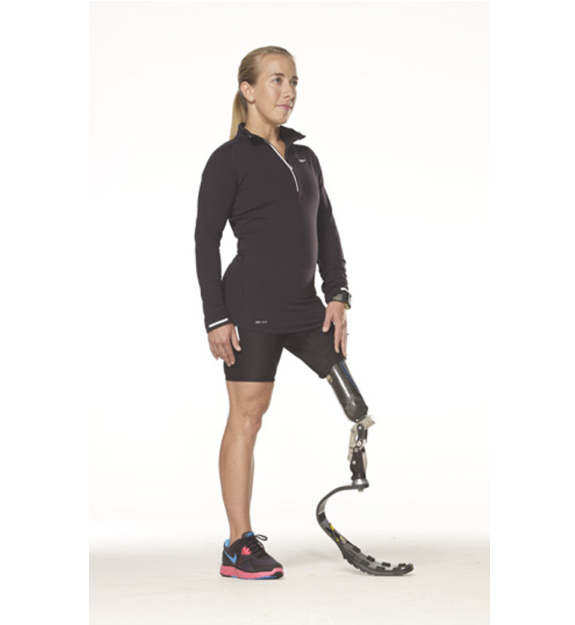
\includegraphics[width=\textwidth]{figures/prosthetic_leg.pdf}
        \caption{Prosthetic leg, Össur Flex-Run}
        \label{fig:prosthetic_leg}
    \end{subfigure}
    \centering
    \begin{subfigure}[b]{0.3\textwidth}
        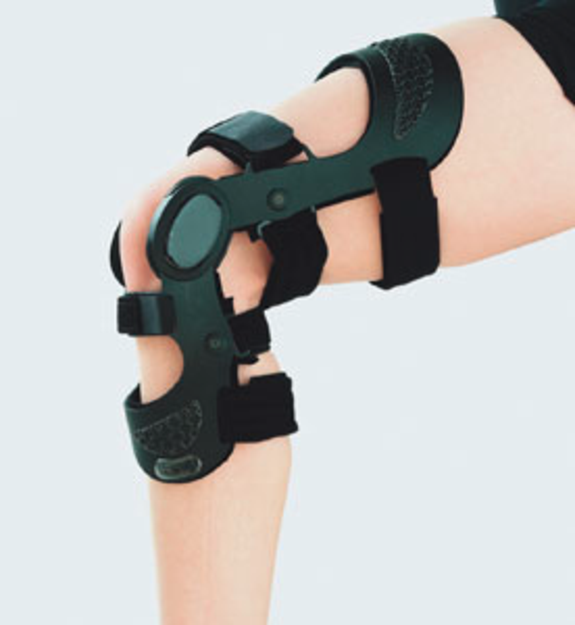
\includegraphics[width=\textwidth]{figures/orthotic_leg.pdf}
        \caption{Knee orthosis, New Hope Co.}
        \label{fig:orthotic_leg}
    \end{subfigure}
    \centering
    \begin{subfigure}[b]{0.3\textwidth}
        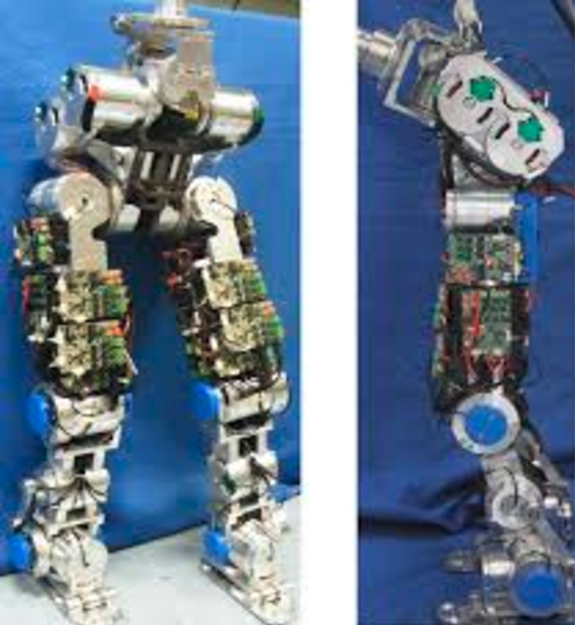
\includegraphics[width=\textwidth]{figures/robotic_leg.pdf}
        \caption{Robotic legs, COMAN robot \cite{coman}}
        \label{fig:robotic_leg}
    \end{subfigure}
\end{figure}

\paragraph{Artificial legged locomotion} % (fold)
\label{par:humanoid_robots}  
The first artificial walking artifacts recorded date from the ancient Greece.
It is in this period when humankind first tries to imitate and replicate the structures found in nature, creating mechanisms to get a deeper knowledge of their functioning and mimic them.
But it is during the Renaissance in Europe when the developments in mechanics and the study of the nature and the human body allows to create the first automata able to walk as a predefined combination of complex mechanical operations.
It is after the Second World War, with the application of electronics and computer technology that the advancement of walking machines is revolutionized \cite{legged_mot_history1}.

The engineering branch of modern robotics has its origins in the second half of the 20th century has a conjunction of the areas of electrical and mechanical engineering and computer science.
However, its interest in achieving resemblance to the locomotion means of both humans and animals  and their capabilities arose in the 1980's.
It first crystallized into the construction of Wabot-1 at WASEDA University or the creation of the Leg Laboratory by Marc Raibert at the Massachusetts Technological Institute.
The purpose of the research in this field was the construction of useful knowledge basis on how human and animal locomotion works that could be used in the creation of legged vehicles, as described in \cite{mit_leg_lab1}.
% paragraph humanoid_robots (end)



% subsection bipedalism_and_engineering (end)

